\documentclass[11pt,preprint, authoryear]{elsarticle}

\usepackage{lmodern}
%%%% My spacing
\usepackage{setspace}
\setstretch{1.2}
\DeclareMathSizes{12}{14}{10}{10}

% Wrap around which gives all figures included the [H] command, or places it "here". This can be tedious to code in Rmarkdown.
\usepackage{float}
\let\origfigure\figure
\let\endorigfigure\endfigure
\renewenvironment{figure}[1][2] {
    \expandafter\origfigure\expandafter[H]
} {
    \endorigfigure
}

\let\origtable\table
\let\endorigtable\endtable
\renewenvironment{table}[1][2] {
    \expandafter\origtable\expandafter[H]
} {
    \endorigtable
}


\usepackage{ifxetex,ifluatex}
\usepackage{fixltx2e} % provides \textsubscript
\ifnum 0\ifxetex 1\fi\ifluatex 1\fi=0 % if pdftex
  \usepackage[T1]{fontenc}
  \usepackage[utf8]{inputenc}
\else % if luatex or xelatex
  \ifxetex
    \usepackage{mathspec}
    \usepackage{xltxtra,xunicode}
  \else
    \usepackage{fontspec}
  \fi
  \defaultfontfeatures{Mapping=tex-text,Scale=MatchLowercase}
  \newcommand{\euro}{€}
\fi

\usepackage{amssymb, amsmath, amsthm, amsfonts}

\def\bibsection{\section*{References}} %%% Make "References" appear before bibliography


\usepackage[round]{natbib}

\usepackage{longtable}
\usepackage[margin=2.3cm,bottom=2cm,top=2.5cm, includefoot]{geometry}
\usepackage{fancyhdr}
\usepackage[bottom, hang, flushmargin]{footmisc}
\usepackage{graphicx}
\numberwithin{equation}{section}
\numberwithin{figure}{section}
\numberwithin{table}{section}
\setlength{\parindent}{0cm}
\setlength{\parskip}{1.3ex plus 0.5ex minus 0.3ex}
\usepackage{textcomp}
\renewcommand{\headrulewidth}{0.2pt}
\renewcommand{\footrulewidth}{0.3pt}

\usepackage{array}
\newcolumntype{x}[1]{>{\centering\arraybackslash\hspace{0pt}}p{#1}}

%%%%  Remove the "preprint submitted to" part. Don't worry about this either, it just looks better without it:
\makeatletter
\def\ps@pprintTitle{%
  \let\@oddhead\@empty
  \let\@evenhead\@empty
  \let\@oddfoot\@empty
  \let\@evenfoot\@oddfoot
}
\makeatother

 \def\tightlist{} % This allows for subbullets!

\usepackage{hyperref}
\hypersetup{breaklinks=true,
            bookmarks=true,
            colorlinks=true,
            citecolor=blue,
            urlcolor=blue,
            linkcolor=blue,
            pdfborder={0 0 0}}


% The following packages allow huxtable to work:
\usepackage{siunitx}
\usepackage{multirow}
\usepackage{hhline}
\usepackage{calc}
\usepackage{tabularx}
\usepackage{booktabs}
\usepackage{caption}


\newenvironment{columns}[1][]{}{}

\newenvironment{column}[1]{\begin{minipage}{#1}\ignorespaces}{%
\end{minipage}
\ifhmode\unskip\fi
\aftergroup\useignorespacesandallpars}

\def\useignorespacesandallpars#1\ignorespaces\fi{%
#1\fi\ignorespacesandallpars}

\makeatletter
\def\ignorespacesandallpars{%
  \@ifnextchar\par
    {\expandafter\ignorespacesandallpars\@gobble}%
    {}%
}
\makeatother

\newlength{\cslhangindent}
\setlength{\cslhangindent}{1.5em}
\newenvironment{CSLReferences}%
  {\setlength{\parindent}{0pt}%
  \everypar{\setlength{\hangindent}{\cslhangindent}}\ignorespaces}%
  {\par}


\urlstyle{same}  % don't use monospace font for urls
\setlength{\parindent}{0pt}
\setlength{\parskip}{6pt plus 2pt minus 1pt}
\setlength{\emergencystretch}{3em}  % prevent overfull lines
\setcounter{secnumdepth}{5}

%%% Use protect on footnotes to avoid problems with footnotes in titles
\let\rmarkdownfootnote\footnote%
\def\footnote{\protect\rmarkdownfootnote}
\IfFileExists{upquote.sty}{\usepackage{upquote}}{}

%%% Include extra packages specified by user

%%% Hard setting column skips for reports - this ensures greater consistency and control over the length settings in the document.
%% page layout
%% paragraphs
\setlength{\baselineskip}{12pt plus 0pt minus 0pt}
\setlength{\parskip}{12pt plus 0pt minus 0pt}
\setlength{\parindent}{0pt plus 0pt minus 0pt}
%% floats
\setlength{\floatsep}{12pt plus 0 pt minus 0pt}
\setlength{\textfloatsep}{20pt plus 0pt minus 0pt}
\setlength{\intextsep}{14pt plus 0pt minus 0pt}
\setlength{\dbltextfloatsep}{20pt plus 0pt minus 0pt}
\setlength{\dblfloatsep}{14pt plus 0pt minus 0pt}
%% maths
\setlength{\abovedisplayskip}{12pt plus 0pt minus 0pt}
\setlength{\belowdisplayskip}{12pt plus 0pt minus 0pt}
%% lists
\setlength{\topsep}{10pt plus 0pt minus 0pt}
\setlength{\partopsep}{3pt plus 0pt minus 0pt}
\setlength{\itemsep}{5pt plus 0pt minus 0pt}
\setlength{\labelsep}{8mm plus 0mm minus 0mm}
\setlength{\parsep}{\the\parskip}
\setlength{\listparindent}{\the\parindent}
%% verbatim
\setlength{\fboxsep}{5pt plus 0pt minus 0pt}



\begin{document}



\begin{frontmatter}  %

\title{Application of PCA and PVCA to a portfolio of 20 stocks in South
Africa}

% Set to FALSE if wanting to remove title (for submission)




\author[Add1]{Wouter Bezuidenhout}
\ead{20088418@sun.ac.za}





\address[Add1]{Stellenbosch Univeristy, South Africa}


\begin{abstract}
\small{
This paper investigates two dimension reduction topics: principal
component analysis and principal variance component analysis. The
techniques are applied to a portfolio of 20 blue chip South African
stocks for the period from 2013/01/01 - 2021/10/29. The importance of
the paper is methodological, specifically the application of PVCA to the
South African Market.
}
\end{abstract}

\vspace{1cm}


\begin{keyword}
\footnotesize{
Principal Component Analysis \sep Principal Variance Component
Analysis \\
\vspace{0.3cm}
}
\footnotesize{
\textit{JEL classification} C38 \sep C58
}
\end{keyword}



\vspace{0.5cm}

\end{frontmatter}



%________________________
% Header and Footers
%%%%%%%%%%%%%%%%%%%%%%%%%%%%%%%%%
\pagestyle{fancy}
\chead{}
\rhead{}
\lfoot{}
\rfoot{\footnotesize Page \thepage}
\lhead{}
%\rfoot{\footnotesize Page \thepage } % "e.g. Page 2"
\cfoot{}

%\setlength\headheight{30pt}
%%%%%%%%%%%%%%%%%%%%%%%%%%%%%%%%%
%________________________

\headsep 35pt % So that header does not go over title




\hypertarget{introduction}{%
\section{\texorpdfstring{Introduction
\label{Introduction}}{Introduction }}\label{introduction}}

Elementary analysis of financial returns usually assume time-invariant
or constant covariances (volatility), known as homoskedasticity. It is
well-known that financial returns posses conditional heteroskedastic, or
time-varying conditional covariances, known as volatility {[}tsay2{]}.
The pursuit of modeling conditional heteroskedasticity is important, and
resulted in a Nobel Prize for Robert Engle. My paper extends this idea
to argue that is more useful to known if volatility is common between
different time-series. The challenge with multivariate volatility
modeling is the growth in dimensions. For K variables, the covariance
matrix has K(K+1)/2 processes to estimate. Therefore, I implement two
dimension reduction techniques to engage a more manageable set of
estimates. I use two methods to explore this: a principal component
analysis (PCA) and a principal variance component analysis (PVCA).

PCA finds structure in the covariance matrix to locate low-dimensional
sub-spaces that contain most of the variation of the data {[}ruppert{]}.
PCA is not feature selection, as each PCA is just a linear combination
of all original variables. PCA is especially useful for highly
correlated variables like financial returns, as PCAs are uncorrelated
from one another. An example of how this is useful, say an analyst would
be interested in the behavior of an index with 50 stocks. After
implementing PCA, the analyst could focus on prediction of a dozen PCAs
responsible for more than 90 percent of the variation in the data,
instead of focusing on all 50 stocks simultaneously
(\protect\hyperlink{ref-ruppert}{Ruppert \& Matteson, 2011}). On the
other hand, PVCA is a generalization of PCA to detect common volatility
factors in returns. The aim of PVCA is to find a small number of common
volatility components in order to find a linear combination of the
series with no conditional heteroscedasticity {[}hu{]}.

The computation required for PVCA is strenuous, and to keep a positive
semi-definite matrix is difficult as dimensions grow. In
\protect\hyperlink{ref-hu}{Hu \& Tsay}
(\protect\hyperlink{ref-hu}{2014}), the author uses 7 currencies,
whereas in \protect\hyperlink{ref-engle}{Engle \& Susmel}
(\protect\hyperlink{ref-engle}{1993}), the author uses 18 indexes.
Therefore, for my application, I have decided to apply these techniques
to a portfolio of 20 blue chip stocks listed on the JSE. My aim is the
showcasing of the two methodologies applied to equity returns. The paper
is structured as follows. Section \ref{Meth} discusses the methodologies
for PCA and PVCA in detail so that the paper is as self-contained as
possible. Section \ref{Data} discusses the data's properties and
transformations implemented. Section \ref{Results} discusses the results
of the two methods. Section \ref{Conclusion} concludes.

\hypertarget{methodologies}{%
\section{\texorpdfstring{Methodologies
\label{Meth}}{Methodologies }}\label{methodologies}}

Data is required to look as follows: one needs a sample
\(\mathbf{Y}_i = (Y_{i,1},..., Y_{i,d}), i=1,...,n\) of d-dimensional
random vectors with mean vector \(\mathbf{\mu}\) and covariance matrix
\(\mathbf{\Sigma}\). PCA is focused on extracting structure from the
covariance matrix. PCA produces zero contemporaneous correlations,
meaning PCA overlooks the dynamic dependence between the volatility
processes (\protect\hyperlink{ref-ISLR}{James, Witten, Hastie \&
Tibshirani, 2013}). PVCA focuses on the dynamic dependence of
volatility. The motivation with PVCA is with a small number of common
volatility components, one can find a linear combinations of the return
series that contains no conditional heteroscedasticity {[}hu{]}. In PCA,
one performs a spectral decomposition of the covariance matrix.
Following \protect\hyperlink{ref-hu}{Hu \& Tsay}
(\protect\hyperlink{ref-hu}{2014}), the authors extend this to propose a
sample estimate of a cumulative generalized kurtosis matrix to summarize
the dynamic volatility dependence of the multivariate time series.
Spectral analysis of this generalized matrix is then used to define
PVCs. In order to determine that no conditional heteroscedasticity is
present in the PVC process, the authors conduct a generalized Ling--Li
test statistic. It is worth noting that
\protect\hyperlink{ref-engle}{Engle \& Susmel}
(\protect\hyperlink{ref-engle}{1993}) conducted a study with a similar
aim, but used noticeably different methods.
\protect\hyperlink{ref-engle}{Engle \& Susmel}
(\protect\hyperlink{ref-engle}{1993}) conducted a pairwise procedure to
test for no conditional heteroscedasticity after modeling using GARCH
and M-GARCH models.

\hypertarget{data}{%
\section{\texorpdfstring{Data \label{Data}}{Data }}\label{data}}

The return series that I have chosen for my application is a portfolio
of 20 blue chip, large cap equities listed on the Johannesburg Stock
Exchange (JSE). The sample period is from 2013/01/01 to 2021/10/29. The
return series has been logged. The following 20 stocks are in the
portfolio. I initially tried to conduct this with the ALSI Top 40, but
there are numerous nuances with such an application that require further
thinking in order to achieve.

\begin{table}[h!]
\centering
\begin{tabular}{|c c|}
\hline
Short name (ticker) & Sector \\
\hline\hline 
BHP Group (BHP) & Resources \\
Anglo American (AGL) & Resources \\
Sasol (SOL) & Resources \\
Anglogold Ashanti (ANG) & Resources \\
Richemont (CFR) & Industrials \\
MTN Group (MTN) & Industrials \\
Shoprite (SHP) & Industrials \\
Mondi (MNP) & Industrials \\
Aspen Pharmaceuticals (APN) & Industrials \\
Naspers (NPN) & Industrials \\
Vodacom (VOD) & Industrials \\
Standard Bank (SBK) & Financials \\
Firstrand (FSR) & Financials \\
ABSA (ABG) & Financials \\
Growthpoint (GRT) & Financials \\
Nedbank (NED) & Financials \\
Investec Ltd. (INL) & Financials \\
Investec Plc. (INP) & Financials \\
Remgro (REM) & Financials \\
Sanlam (SLM) & Financials \\ [1ex] 
\hline
\end{tabular}
\caption{Portfolio of 20 stocks}
\end{table}

In order to get an idea of the series, I plot them below. Figure
\ref{Figure_1} shows no noticeable missing periods of data, furthermore,
one can already see periods of high variance in some stock returns.
There is a period in 2020 where Sasol (SOL) shows especially high
variance. In the next section, I run the PCA and PVCA, and discuss their
results.

\begin{figure}[!htb]
\centering
\includegraphics[scale=0.6]{figures/Figure_1.jpeg}
\caption{Stock returns of the portoflio}\label{Figure_1}
\end{figure}

\hypertarget{results}{%
\section{\texorpdfstring{Results
\label{Results}}{Results }}\label{results}}

\hypertarget{principal-component-analysis}{%
\subsection{Principal Component
Analysis}\label{principal-component-analysis}}

It is recommended to standardize the variables when one conducts PCA. If
variables are on different scales, then variables with greater variance
in magnitude will dominate the analysis and therefore bias the results
(\protect\hyperlink{ref-ISLR}{James, Witten, Hastie \& Tibshirani,
2013}). In my case, with logged returns, it should not be necessary, but
I do so for completeness. Furthermore, I check for missing returns and
find a small amount in Anglogold Ashanti (ANG) and Aspen Pharmaceuticals
(APN). I impute these by drawing from their distribution. I calculate
the PCAs using the prcomp function in R from the stats package. This
function decomposes the d-dimensional into d contemporaneously
uncorrelated PCAs, and ranks them based on the amount of variability
explained by each. Figure \ref{Figure_2} displays the scree plot of the
PCAs. A scree plot shows the amount of variability explained by each
PCA. There are 20 PCAs, but I have chosen to display the first 12. The
first PCA explains 36,5 percent of the variability of all 20 stock
returns. To complement this, Table \ref{Table_1} shows the cumulative
proportions of variance explained by each PCA. With 11 PCAs, one can
explain more than 90 percent of the variance in the portfolio of 20
stock returns. Figure \ref{Figure_3} takes a closer look at PCA 1 to
understand which shares underlie its importance. The figure shows that
Sasol (SOL) represents most of the contribution, followed by Nedbank
(NED), Absa (ABG), Firstrand (FSR), MTN and Standard Bank (SBK).

\begin{figure}[!tbp]
\centering
\begin{minipage}[b]{7cm}
\includegraphics[scale=0.45]{figures/Figure_2.jpeg}
\caption{Scree plot fo PCAs}\label{Figure_2}
\end{minipage}
\hspace{0.05cm}
\hfill
\begin{minipage}[b]{7cm}
\includegraphics[scale = 0.45]{figures/Figure_3.jpeg}
\caption{Individual contributions to PCA 1}\label{Figure_3}
\end{minipage}
\hspace{0.1cm}
\hfill
\end{figure}

\begin{table}[h!]
\centering
\begin{tabular}{|c c c c c c c c c c c c c|}
\hline
Category & PC1 & PC2 & PC3 & PC4 & PC5 & PC6 & PC7 & PC8 & PC9 & PC10 & PC11 & PC12 \\
\hline\hline 
Eigenvalues & 43,3 & 30,3 & 21,6 & 13,4 & 10,3 & 8,4 & 7,2 & 6,4 & 3,5 & 2,4 & 1,8 & 1,6 \\
Prop of Variance (\%) & 36,5 & 12,5 & 9,2 & 7,1 & 5 & 4,6 & 4,1 & 4 & 3 & 2,2 & 2,1 & 1,6 \\
Cum Prop (\%) & 36,5 & 49 & 58,3 & 65,4 & 70,4 & 75 & 79,1 & 83,2 & 86,1 & 88,3 & 90,4 & 92,1 \\ 
\hline
\end{tabular}
\caption{Importance of PCAs}\label{Table_1}
\end{table}

For a deeper look at the PCAs, it is worth investigating the
eigenvectors. Appendix Table \ref{Appendix_1} shows the eigenvectors for
each PCA. Following the approach of
\protect\hyperlink{ref-ruppert}{Ruppert \& Matteson}
(\protect\hyperlink{ref-ruppert}{2011}), the first eigenvector has only
negative values, meaning for an increase in PCA 1 all returns should
decrease. Eigenvector 2 has 7 negative values and 13 positive values,
where the negative values are all four resources stocks, as well as the
following industrials: Naspers, Mondi and Richemont. Variation along
this eigenvector has resource stocks and three industrials moving in the
opposite direction to other returns. It is not uncommon to see resource
move opposite to the market, and therefore this PCA accounts for 12,5\%
of variation. For eigenvector three, all values are negative except for
Anglo American, BHP, Richemont, Investec Ltd, Investec Plc, Mondi and
Sasol. This PCA accounts for 9,2\% of the variation. Both PCA 2 and 3
should not be over-confidently interpreted, but rather modeled
quantitatively. In conclusion to the PCAs, logically, it seems that
sectors have common variation and that PCA 1 represents an overall
market factor. The PCAs derived are now able to be used in prediction
modeling by an analyst who will now have less dimensions to work with
opposed to having to work with all 20 stocks. There is no golden rule
about how many PCAs to use, but I argue that 90 percent of variation
explained by 11 PCAs is suitable. For interest sake, if I modeled stocks
only from the same sector (say Resources), one would observe the 90
percent threshold reached in a handful of PCAs opposed to a dozen. In
the next subsection, I turn to the results of the PVCA.

\hypertarget{principal-variance-component-analysis}{%
\subsection{Principal Variance Component
Analysis}\label{principal-variance-component-analysis}}

\protect\hyperlink{ref-hu}{Hu \& Tsay}
(\protect\hyperlink{ref-hu}{2014}) proposed the idea of PVCA, the
generalization of PCA methods to focus more directly on modeling common
multivariate volatility. The method requires the specification of a
Vector-autoregression (VAR) model to account for serial correlation.
According to the Akaike Information Criterion, my data requires only two
lags where as in \protect\hyperlink{ref-hu}{Hu \& Tsay}
(\protect\hyperlink{ref-hu}{2014}), the authors uses 5 lags. After
running Portmanteau tests to detect serial correlation, I am not
completely satisfied that serial correlation is not present, however, no
additional amount of lags remove this. Additionally, the data has been
logged and differenced (working with returns), and therefore I proceed.

After running the model and producing 20 PVCAs, I conduct univariate
ARCH tests on all 20 PVCAs. I find that the 19th PVCA has no conditional
heteroscedasticity. In the \protect\hyperlink{ref-hu}{Hu \& Tsay}
(\protect\hyperlink{ref-hu}{2014}) paper, this result was found with
their seventh of seven currencies. This implies that there certainly
exists common volatility factors in my portfolio of 20 stocks
(\protect\hyperlink{ref-hu}{Hu \& Tsay, 2014}). Figure \ref{Figure_6}
presents the time series of selected PVCAs. Although, the F-Tests
confirm no conditional heteroscedasticity, the variances do not look
much different with the eye. Additional ACF plots are not informative
either.

\begin{figure}[!htb]
\centering
\includegraphics[scale=.45]{figures/Figure_6.jpeg}
\caption{Time Series of selected PVCAs}\label{Figure_6}
\end{figure}

Figure \ref{Figure_4} displays the scree plot of the PVCAs. In this
case, the scree plot shows the amount of volatility explained by each
PVCA. The first PVCA explains 27,7 percent, the second 19,4 percent and
the third 13,8 percent, of the volatility of all 20 stock returns.
Cumulatively, the first three PVCAs account for 61 percent of
volatility. Table \ref{Table_1} shows the cumulative proportions of
volatility explained by each PVCA more specifically. With 12 PVCAs, one
can explain 96,2 percent of the volatility in the portfolio of 20 stock
returns. Figure \ref{Figure_5} takes a closer look at PVCA 1 to
understand which shares underlie its importance. The figure shows that
Anglo American (ANG) and Shoprite (SHP) are most important in the first
PVCA. This is a surprising result. In order to understand the PVCAs
better, I turn to looking at their eigenvectors.

Table \ref{Figure_3} in the appendix contains the eigenvectors for the
individual stocks for the first 12 PVCAs (explaining 96\% of
volatility). Note that I have rounded off for the values for
presentability. If the F-test for conditional heteroscedasticity not
present at PVCA 19, then my interpretation is that the first 18 PVCAs
account for all the common and time-varying volatility, whereafter the
19th PVCA shows time-invariant covariance. Overall, the PVCA model is a
good attempt at a unique method to modeling common volatility.
Additionally, a more interesting application might highlight the
usefulness of the method more. \protect\hyperlink{ref-hu}{Hu \& Tsay}
(\protect\hyperlink{ref-hu}{2014}) had 7 variables in their sample,
whereas I have 20, and \protect\hyperlink{ref-engle}{Engle \& Susmel}
(\protect\hyperlink{ref-engle}{1993}) had 18 - although
\protect\hyperlink{ref-engle}{Engle \& Susmel}
(\protect\hyperlink{ref-engle}{1993}) used vastly different methods. In
my calculations, as one added more variables, the process immediately
became more complex computationally and mathematically.

\begin{table}[h!]
\centering
\begin{tabular}{|c c c c c c c c c c c c c|}
\hline
PVCA & 1 & 2 & 3 & 4 & 5 & 6 & 7 & 8 & 9 & 10 & 11 & 12 \\
\hline\hline 
Eigenvalues & 43,3 & 30,3 & 21,6 & 13,4 & 10,3 & 8,4 & 7,2 & 6,4 & 3,5 & 2,4 & 1,8 & 1,6 \\
Prop of Volatility (\%) & 27,7 & 19,4 & 13,8 & 8,5 & 6,6 & 5,4 & 4,6 & 4,1 & 2,3 & 1,6 & 1,2 & 1 \\ 
Cum Prop (\%) & 27,7 & 47,1 & 60,9 & 69,4 & 76 & 81,4 & 86 & 90,1 & 92,4 & 94 & 95,2 & 96,2 \\ 
\hline
\end{tabular}
\caption{PVCAs}\label{Table_2}
\end{table}

\begin{figure}[!htb]
\centering
\includegraphics[scale=.45]{figures/Figure_4.jpeg}
\caption{PVCAs proportions explained}\label{Figure_4}
\end{figure}

\begin{figure}[!htb]
\centering
\includegraphics[scale=.45]{figures/Figure_5.jpeg}
\caption{Individual contributions to PVCA 1}\label{Figure_5}
\end{figure}

\hypertarget{conclusion}{%
\section{\texorpdfstring{Conclusion
\label{Conclusion}}{Conclusion }}\label{conclusion}}

Modelling common volatility has been the pursuit of numerous authors in
the past. Options traders are often concerned with modelling common
implied volatility, too. However, the challenge with multivariate
volatility modeling is the growth in dimensions of parameters required
to be estimated. For K variables, the covariance matrix has K(K+1)/2
processes to estimate. Dimension reduction techniques are therefore
crucial if one is to build a model that is accurate and efficient. In
this paper, I have implemented two dimension reduction techniques, a
principal component analysis and a principal variance component
analysis. PCA is concerned with investigating the structure of
covariance matrix in order to represent the high-dimensional series with
a low-dimensional uncorrelated PCAs. PVCAs generalize the process of
PCAs by estimating a cumulative generalized kurtosis matrix to summarize
the dynamic volatility dependence of the multivariate time series. The
motivation of PVCAs is to find a PVCA combination that is a linear
combinations of the return series that contains no conditional
heteroscedasticity.

My PCA model was successful and it logically it seemed that sectors were
moving together within the PCA. With 12 PCAs, my model could account for
more than 92 percent of the variation of the 20-stock portfolio. The
noticeable contributions to explaining variation within PCA 1 were
Sasol, Nedbank, Absa, Firstrand, MTN and Standard Bank. This PCA is
ready to be used in further analysis. The PVCA model was a good attempt
at a unique method to modelling common volatility. The first 12 PVCAs
account for 96,2 percent of the volatility. The F-tests that I conducted
to test for the presence of conditional heteroscedasticity showed that
PVCA 19 had no conditional heteroscedasticity. This means that the
common volatility was accounted for in the previous PVCAs. Surprisingly,
in the first PVCA, Anglo American and Shoprite were the most important
contributors. In conclusion, more work needs to be done to elaborate on
the R-package that models PVCA and a more suitable application needs to
be conducted to really test the usefulness of the method.

\newpage

\hypertarget{references}{%
\section*{References}\label{references}}
\addcontentsline{toc}{section}{References}

\hypertarget{refs}{}
\begin{CSLReferences}{1}{0}
\leavevmode\hypertarget{ref-engle}{}%
Engle, R.F. \& Susmel, R. 1993. Common volatility in international
equity markets. \emph{Journal of Business \& Economic Statistics}.
11(2):167--176.

\leavevmode\hypertarget{ref-hu}{}%
Hu, Y.-P. \& Tsay, R.S. 2014. Principal volatility component analysis.
\emph{Journal of Business \& Economic Statistics}. 32(2):153--164.

\leavevmode\hypertarget{ref-ISLR}{}%
James, G., Witten, D., Hastie, T. \& Tibshirani, R. 2013. \emph{An
introduction to statistical learning}. Vol. 112. Springer.

\leavevmode\hypertarget{ref-Texevier}{}%
Katzke, N.F. 2017. \emph{{Texevier}: {P}ackage to create elsevier
templates for rmarkdown}. Stellenbosch, South Africa: Bureau for
Economic Research.

\leavevmode\hypertarget{ref-ruppert}{}%
Ruppert, D. \& Matteson, D.S. 2011. \emph{Statistics and data analysis
for financial engineering}. Vol. 13. Springer.

\leavevmode\hypertarget{ref-tsay2}{}%
Tsay, R.S. 2013. \emph{Multivariate time series analysis: With r and
financial applications}. John Wiley \& Sons.

\leavevmode\hypertarget{ref-tsay}{}%
Tsay, R.S. 2014. \emph{An introduction to analysis of financial data
with r}. John Wiley \& Sons.

\end{CSLReferences}

\newpage

\hypertarget{appendix}{%
\section*{Appendix}\label{appendix}}
\addcontentsline{toc}{section}{Appendix}

\hypertarget{appendix-a}{%
\subsection*{Appendix A}\label{appendix-a}}
\addcontentsline{toc}{subsection}{Appendix A}

\begin{figure}[!htb]
\centering
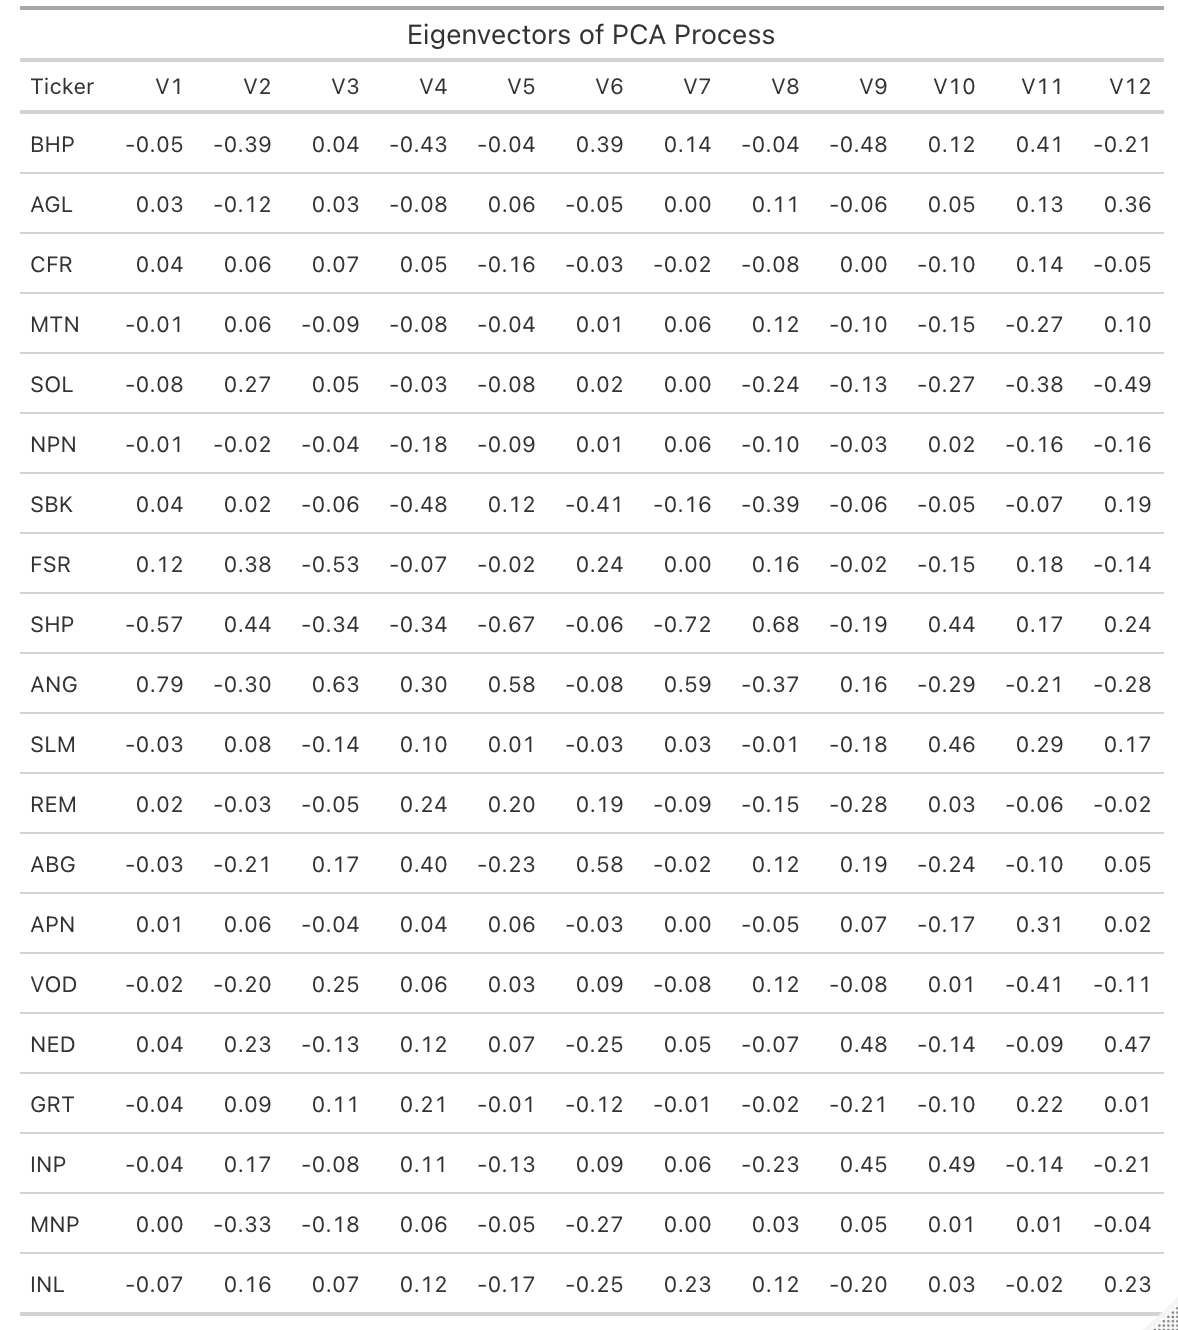
\includegraphics[scale=0.3]{figures/Table_2.png}
\caption{Eigenvectors of PCAs}\label{Appendix_1}
\end{figure}

\begin{figure}[!htb]
\centering
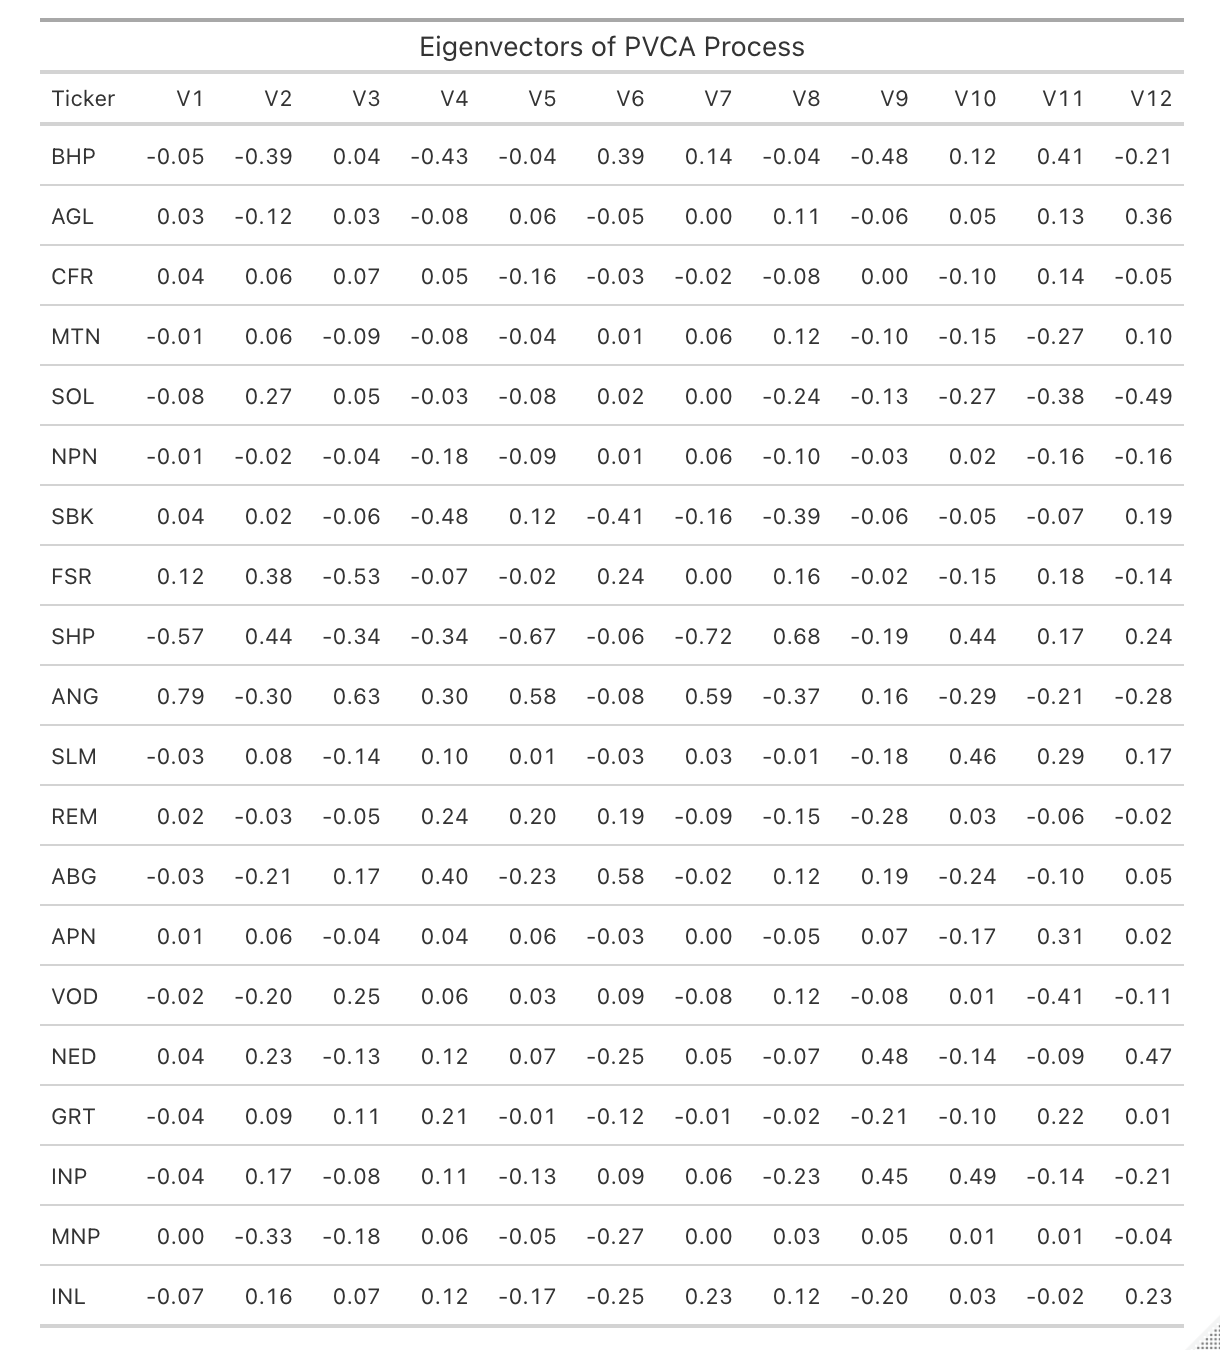
\includegraphics[scale=0.3]{figures/Table_1.png}
\caption{Eigenvectors of PVCA}\label{Table_3}
\end{figure}

\bibliography{Tex/ref}





\end{document}
